%%%%%%%%%%%%%%%%%%%%%%%%%%%%%%%%%%%%%%%%%%%%%%%%%%%%%%%%%%%%%%%%%%%%%%%%%%%%%%%%%%%%%%%%%%%%%%%%%
%
% Document:     Data Management  product tree
%
%%%%%%%%%%%%%%%%%%%%%%%%%%%%%%%%%%%%%%%%%%%%%%%%%%%%%%%%%%%%%%%%%%%%%%%%%%%%%%
\documentclass{article}
\usepackage{times,layouts}
\usepackage{tikz,hyperref,amsmath}
\usetikzlibrary{positioning,arrows,shapes,decorations.shapes,shapes.arrows}
\usetikzlibrary{backgrounds,calc}
\usepackage[paperwidth=1647.9999999999998pt,paperheight=516pt,
left=-2mm,top=3mm,bottom=0mm,right=0mm,
noheadfoot,marginparwidth=0pt,includemp=false,
textwidth=30cm,textheight=50mm]{geometry}
\newcommand\showpage{%
\setlayoutscale{0.5}\setlabelfont{\tiny}\printheadingsfalse\printparametersfalse
\currentpage\pagedesign}
\hypersetup{pdftitle={Data Management products }, pdfsubject={Diagram illustrating the
                products in LSST Data Management }, pdfauthor={Extracted from MagicDraw}}
\tikzstyle{tbox}=[rectangle,text centered, text width=30mm]
\tikzstyle{wbbox}=[rectangle, rounded corners=3pt, draw=black, top color=blue!50!white,
                    bottom color=white, very thick, minimum height=40pt, inner sep=2pt,
                    text centered, text width=30mm]
\tikzstyle{pbox}=[rectangle, rounded corners=3pt, draw=black, top
 color=yellow!50!white, bottom color=white, very thick,
 minimum height=36pt, inner sep=3pt, text centered, text width=35mm]
\tikzstyle{pline}=[-, thick]
\begin{document}
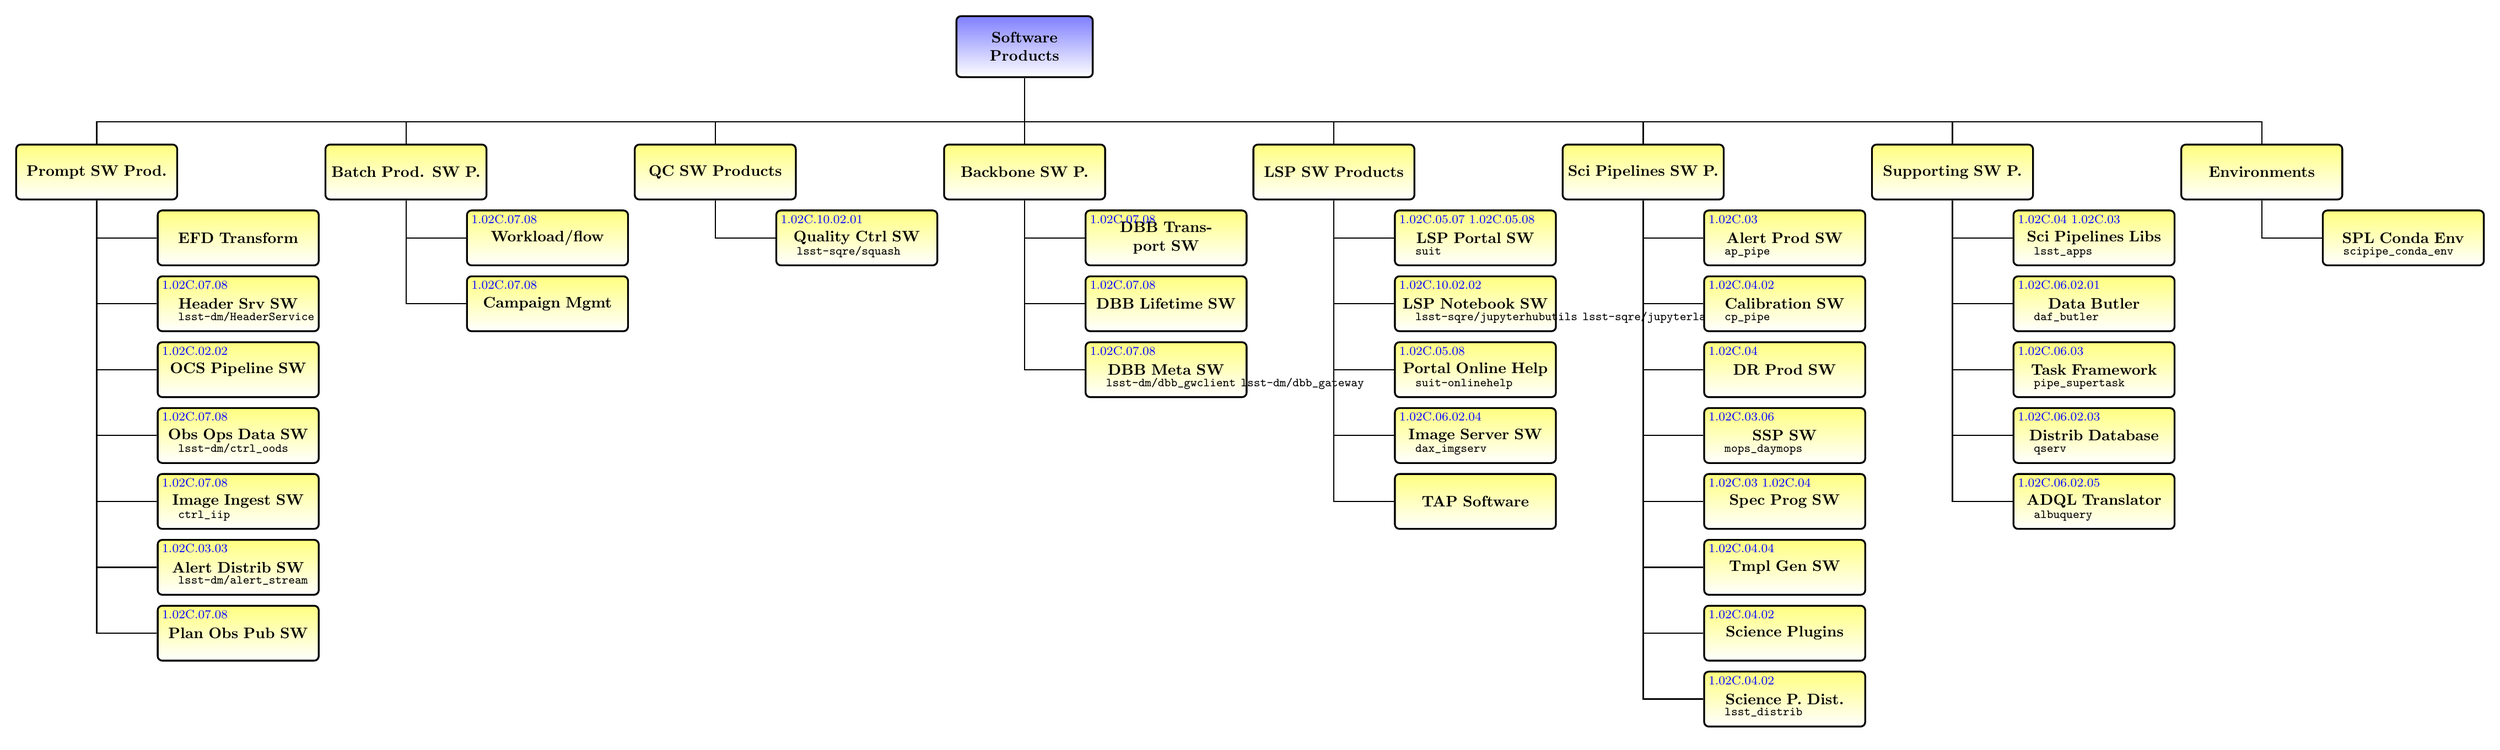
\begin{tikzpicture}[node distance=0mm]


\node (PRSW) [pbox, 
] {\textbf{Prompt SW Prod.
} };\node [below right] at (PRSW.north west) {\footnotesize \color{blue}} ;

\node (EFDT) [pbox,below right=6pt and -14pt of PRSW] {\textbf{EFD Transform
} };\node [below right] at (EFDT.north west) {\footnotesize \color{blue}} ;

 \draw[pline] (PRSW.south) -| ++(0,0) |- (EFDT.west); 
\node (HEADER) [pbox,below=6pt of EFDT] {\textbf{Header Srv SW
} };\node [below right] at (HEADER.north west) {\footnotesize \color{blue}1.02C.07.08} ;
\node (HEADERpkg) [tbox,below=3mm of HEADER.north] {{\footnotesize \color{black} \begin{verbatim} lsst-dm/HeaderService \end{verbatim} }  };

 \draw[pline] (PRSW.south) -| ++(0,0) |- (HEADER.west); 
\node (OCPS) [pbox,below=6pt of HEADER] {\textbf{OCS Pipeline SW
} };\node [below right] at (OCPS.north west) {\footnotesize \color{blue}1.02C.02.02} ;

 \draw[pline] (PRSW.south) -| ++(0,0) |- (OCPS.west); 
\node (OODS) [pbox,below=6pt of OCPS] {\textbf{Obs Ops Data SW
} };\node [below right] at (OODS.north west) {\footnotesize \color{blue}1.02C.07.08} ;
\node (OODSpkg) [tbox,below=3mm of OODS.north] {{\footnotesize \color{black} \begin{verbatim} lsst-dm/ctrl_oods \end{verbatim} }  };

 \draw[pline] (PRSW.south) -| ++(0,0) |- (OODS.west); 
\node (IIP) [pbox,below=6pt of OODS] {\textbf{Image Ingest SW
} };\node [below right] at (IIP.north west) {\footnotesize \color{blue}1.02C.07.08} ;
\node (IIPpkg) [tbox,below=3mm of IIP.north] {{\footnotesize \color{black} \begin{verbatim} ctrl_iip \end{verbatim} }  };

 \draw[pline] (PRSW.south) -| ++(0,0) |- (IIP.west); 
\node (ALRTDSTR) [pbox,below=6pt of IIP] {\textbf{Alert Distrib SW
} };\node [below right] at (ALRTDSTR.north west) {\footnotesize \color{blue}1.02C.03.03} ;
\node (ALRTDSTRpkg) [tbox,below=3mm of ALRTDSTR.north] {{\footnotesize \color{black} \begin{verbatim} lsst-dm/alert_stream \end{verbatim} }  };

 \draw[pline] (PRSW.south) -| ++(0,0) |- (ALRTDSTR.west); 
\node (OBSPUB) [pbox,below=6pt of ALRTDSTR] {\textbf{Plan Obs Pub SW
} };\node [below right] at (OBSPUB.north west) {\footnotesize \color{blue}1.02C.07.08} ;

 \draw[pline] (PRSW.south) -| ++(0,0) |- (OBSPUB.west); 
\node (BPSWP) [pbox, 
right=96pt of PRSW] {\textbf{Batch Prod. SW P.
} };\node [below right] at (BPSWP.north west) {\footnotesize \color{blue}} ;

\node (WLWF) [pbox,below right=6pt and -14pt of BPSWP] {\textbf{Workload/flow
} };\node [below right] at (WLWF.north west) {\footnotesize \color{blue}1.02C.07.08} ;

 \draw[pline] (BPSWP.south) -| ++(0,0) |- (WLWF.west); 
\node (CMPGN) [pbox,below=6pt of WLWF] {\textbf{Campaign Mgmt
} };\node [below right] at (CMPGN.north west) {\footnotesize \color{blue}1.02C.07.08} ;

 \draw[pline] (BPSWP.south) -| ++(0,0) |- (CMPGN.west); 
\node (QCSWP) [pbox, 
right=96pt of BPSWP] {\textbf{QC SW Products
} };\node [below right] at (QCSWP.north west) {\footnotesize \color{blue}} ;

\node (QCSW) [pbox,below right=6pt and -14pt of QCSWP] {\textbf{Quality Ctrl SW
} };\node [below right] at (QCSW.north west) {\footnotesize \color{blue}1.02C.10.02.01} ;
\node (QCSWpkg) [tbox,below=3mm of QCSW.north] {{\footnotesize \color{black} \begin{verbatim} lsst-sqre/squash \end{verbatim} }  };

 \draw[pline] (QCSWP.south) -| ++(0,0) |- (QCSW.west); 
\node (BBSWP) [pbox, 
right=96pt of QCSWP] {\textbf{Backbone SW P.
} };\node [below right] at (BBSWP.north west) {\footnotesize \color{blue}} ;

\node (DBBTR) [pbox,below right=6pt and -14pt of BBSWP] {\textbf{DBB Transport SW
} };\node [below right] at (DBBTR.north west) {\footnotesize \color{blue}1.02C.07.08} ;

 \draw[pline] (BBSWP.south) -| ++(0,0) |- (DBBTR.west); 
\node (DBBLIFE) [pbox,below=6pt of DBBTR] {\textbf{DBB Lifetime SW
} };\node [below right] at (DBBLIFE.north west) {\footnotesize \color{blue}1.02C.07.08} ;

 \draw[pline] (BBSWP.south) -| ++(0,0) |- (DBBLIFE.west); 
\node (DBBMD) [pbox,below=6pt of DBBLIFE] {\textbf{DBB Meta SW
} };\node [below right] at (DBBMD.north west) {\footnotesize \color{blue}1.02C.07.08} ;
\node (DBBMDpkg) [tbox,below=3mm of DBBMD.north] {{\footnotesize \color{black} \begin{verbatim} lsst-dm/dbb_gwclient lsst-dm/dbb_gateway \end{verbatim} }  };

 \draw[pline] (BBSWP.south) -| ++(0,0) |- (DBBMD.west); 
\node (LSPSWP) [pbox, 
right=96pt of BBSWP] {\textbf{LSP SW Products
} };\node [below right] at (LSPSWP.north west) {\footnotesize \color{blue}} ;

\node (PRTLSW) [pbox,below right=6pt and -14pt of LSPSWP] {\textbf{LSP Portal SW
} };\node [below right] at (PRTLSW.north west) {\footnotesize \color{blue}1.02C.05.07 1.02C.05.08} ;
\node (PRTLSWpkg) [tbox,below=3mm of PRTLSW.north] {{\footnotesize \color{black} \begin{verbatim} suit \end{verbatim} }  };

 \draw[pline] (LSPSWP.south) -| ++(0,0) |- (PRTLSW.west); 
\node (NBSW) [pbox,below=6pt of PRTLSW] {\textbf{LSP Notebook SW
} };\node [below right] at (NBSW.north west) {\footnotesize \color{blue}1.02C.10.02.02} ;
\node (NBSWpkg) [tbox,below=3mm of NBSW.north] {{\footnotesize \color{black} \begin{verbatim} lsst-sqre/jupyterhubutils lsst-sqre/jupyterlabutils \end{verbatim} }  };

 \draw[pline] (LSPSWP.south) -| ++(0,0) |- (NBSW.west); 
\node (PRTLOH) [pbox,below=6pt of NBSW] {\textbf{Portal Online Help
} };\node [below right] at (PRTLOH.north west) {\footnotesize \color{blue}1.02C.05.08} ;
\node (PRTLOHpkg) [tbox,below=3mm of PRTLOH.north] {{\footnotesize \color{black} \begin{verbatim} suit-onlinehelp \end{verbatim} }  };

 \draw[pline] (LSPSWP.south) -| ++(0,0) |- (PRTLOH.west); 
\node (DAXIMG) [pbox,below=6pt of PRTLOH] {\textbf{Image Server SW
} };\node [below right] at (DAXIMG.north west) {\footnotesize \color{blue}1.02C.06.02.04} ;
\node (DAXIMGpkg) [tbox,below=3mm of DAXIMG.north] {{\footnotesize \color{black} \begin{verbatim} dax_imgserv \end{verbatim} }  };

 \draw[pline] (LSPSWP.south) -| ++(0,0) |- (DAXIMG.west); 
\node (TAPSW) [pbox,below=6pt of DAXIMG] {\textbf{TAP Software
} };\node [below right] at (TAPSW.north west) {\footnotesize \color{blue}} ;

 \draw[pline] (LSPSWP.south) -| ++(0,0) |- (TAPSW.west); 
\node (SCIPSWP) [pbox, 
right=96pt of LSPSWP] {\textbf{Sci Pipelines SW P.
} };\node [below right] at (SCIPSWP.north west) {\footnotesize \color{blue}} ;

\node (APPRMPT) [pbox,below right=6pt and -14pt of SCIPSWP] {\textbf{Alert Prod SW
} };\node [below right] at (APPRMPT.north west) {\footnotesize \color{blue}1.02C.03} ;
\node (APPRMPTpkg) [tbox,below=3mm of APPRMPT.north] {{\footnotesize \color{black} \begin{verbatim} ap_pipe \end{verbatim} }  };

 \draw[pline] (SCIPSWP.south) -| ++(0,0) |- (APPRMPT.west); 
\node (DMCAL) [pbox,below=6pt of APPRMPT] {\textbf{Calibration SW
} };\node [below right] at (DMCAL.north west) {\footnotesize \color{blue}1.02C.04.02} ;
\node (DMCALpkg) [tbox,below=3mm of DMCAL.north] {{\footnotesize \color{black} \begin{verbatim} cp_pipe \end{verbatim} }  };

 \draw[pline] (SCIPSWP.south) -| ++(0,0) |- (DMCAL.west); 
\node (DRP) [pbox,below=6pt of DMCAL] {\textbf{DR Prod SW
} };\node [below right] at (DRP.north west) {\footnotesize \color{blue}1.02C.04} ;

 \draw[pline] (SCIPSWP.south) -| ++(0,0) |- (DRP.west); 
\node (SSP) [pbox,below=6pt of DRP] {\textbf{SSP SW
} };\node [below right] at (SSP.north west) {\footnotesize \color{blue}1.02C.03.06} ;
\node (SSPpkg) [tbox,below=3mm of SSP.north] {{\footnotesize \color{black} \begin{verbatim} mops_daymops \end{verbatim} }  };

 \draw[pline] (SCIPSWP.south) -| ++(0,0) |- (SSP.west); 
\node (SP) [pbox,below=6pt of SSP] {\textbf{Spec Prog SW
} };\node [below right] at (SP.north west) {\footnotesize \color{blue}1.02C.03 1.02C.04} ;

 \draw[pline] (SCIPSWP.south) -| ++(0,0) |- (SP.west); 
\node (TMPLGEN) [pbox,below=6pt of SP] {\textbf{Tmpl Gen SW
} };\node [below right] at (TMPLGEN.north west) {\footnotesize \color{blue}1.02C.04.04} ;

 \draw[pline] (SCIPSWP.south) -| ++(0,0) |- (TMPLGEN.west); 
\node (SPLUG) [pbox,below=6pt of TMPLGEN] {\textbf{Science Plugins
} };\node [below right] at (SPLUG.north west) {\footnotesize \color{blue}1.02C.04.02} ;

 \draw[pline] (SCIPSWP.south) -| ++(0,0) |- (SPLUG.west); 
\node (SPDIST) [pbox,below=6pt of SPLUG] {\textbf{Science P. Dist.
} };\node [below right] at (SPDIST.north west) {\footnotesize \color{blue}1.02C.04.02} ;
\node (SPDISTpkg) [tbox,below=3mm of SPDIST.north] {{\footnotesize \color{black} \begin{verbatim} lsst_distrib \end{verbatim} }  };

 \draw[pline] (SCIPSWP.south) -| ++(0,0) |- (SPDIST.west); 
\node (SPSWP) [pbox, 
right=96pt of SCIPSWP] {\textbf{Supporting SW P.
} };\node [below right] at (SPSWP.north west) {\footnotesize \color{blue}} ;

\node (SCIPIPE) [pbox,below right=6pt and -14pt of SPSWP] {\textbf{Sci Pipelines Libs
} };\node [below right] at (SCIPIPE.north west) {\footnotesize \color{blue}1.02C.04 1.02C.03} ;
\node (SCIPIPEpkg) [tbox,below=3mm of SCIPIPE.north] {{\footnotesize \color{black} \begin{verbatim} lsst_apps \end{verbatim} }  };

 \draw[pline] (SPSWP.south) -| ++(0,0) |- (SCIPIPE.west); 
\node (BUTLER) [pbox,below=6pt of SCIPIPE] {\textbf{Data Butler
} };\node [below right] at (BUTLER.north west) {\footnotesize \color{blue}1.02C.06.02.01} ;
\node (BUTLERpkg) [tbox,below=3mm of BUTLER.north] {{\footnotesize \color{black} \begin{verbatim} daf_butler \end{verbatim} }  };

 \draw[pline] (SPSWP.south) -| ++(0,0) |- (BUTLER.west); 
\node (TXF) [pbox,below=6pt of BUTLER] {\textbf{Task Framework
} };\node [below right] at (TXF.north west) {\footnotesize \color{blue}1.02C.06.03} ;
\node (TXFpkg) [tbox,below=3mm of TXF.north] {{\footnotesize \color{black} \begin{verbatim} pipe_supertask \end{verbatim} }  };

 \draw[pline] (SPSWP.south) -| ++(0,0) |- (TXF.west); 
\node (QSERV) [pbox,below=6pt of TXF] {\textbf{Distrib Database
} };\node [below right] at (QSERV.north west) {\footnotesize \color{blue}1.02C.06.02.03} ;
\node (QSERVpkg) [tbox,below=3mm of QSERV.north] {{\footnotesize \color{black} \begin{verbatim} qserv \end{verbatim} }  };

 \draw[pline] (SPSWP.south) -| ++(0,0) |- (QSERV.west); 
\node (ADQL) [pbox,below=6pt of QSERV] {\textbf{ADQL Translator
} };\node [below right] at (ADQL.north west) {\footnotesize \color{blue}1.02C.06.02.05} ;
\node (ADQLpkg) [tbox,below=3mm of ADQL.north] {{\footnotesize \color{black} \begin{verbatim} albuquery \end{verbatim} }  };

 \draw[pline] (SPSWP.south) -| ++(0,0) |- (ADQL.west); 
\node (ENVS) [pbox, 
right=96pt of SPSWP] {\textbf{Environments
} };\node [below right] at (ENVS.north west) {\footnotesize \color{blue}} ;

\node (SPLCE) [pbox,below right=6pt and -14pt of ENVS] {\textbf{SPL Conda Env
} };\node [below right] at (SPLCE.north west) {\footnotesize \color{blue}} ;
\node (SPLCEpkg) [tbox,below=3mm of SPLCE.north] {{\footnotesize \color{black} \begin{verbatim} scipipe_conda_env \end{verbatim} }  };

 \draw[pline] (ENVS.south) -| ++(0,0) |- (SPLCE.west); 
\node (DMSW) [wbbox, above=43pt of BBSWP]{\textbf{Software Products}};
 \draw[pline]   (PRSW.north) -- ++(0.0,0.5) -| (DMSW.south) ; 
 \draw[pline]   (BPSWP.north) -- ++(0.0,0.5) -| (DMSW.south) ; 
 \draw[pline]   (QCSWP.north) -- ++(0.0,0.5) -| (DMSW.south) ; 
 \draw[pline]   (BBSWP.north) -- ++(0.0,0.5) -| (DMSW.south) ; 
 \draw[pline]   (LSPSWP.north) -- ++(0.0,0.5) -| (DMSW.south) ; 
 \draw[pline]   (SCIPSWP.north) -- ++(0.0,0.5) -| (DMSW.south) ; 
 \draw[pline]   (SPSWP.north) -- ++(0.0,0.5) -| (DMSW.south) ; 
 \draw[pline]   (ENVS.north) -- ++(0.0,0.5) -| (DMSW.south) ; 

\end{tikzpicture}
\end{document}
